\documentclass[a4paper,11pt]{article} 

\usepackage{booktabs}
\usepackage[english]{babel} 
\usepackage[utf8]{inputenc} 
\usepackage[section]{placeins}
\usepackage[T1]{fontenc} 
\usepackage{mathtools} 
\usepackage[table,xcdraw]{xcolor}
\usepackage{siunitx} 
\usepackage{float} 
\usepackage{graphicx} 
\usepackage[justification=centering]{caption} 
\usepackage{subcaption}
\usepackage{wallpaper}
\usepackage{nomencl}
\usepackage{fancyhdr}
\usepackage{url}
\usepackage[hidelinks]{hyperref}
\usepackage[left=3cm,right=3cm,top=3cm,bottom=5cm]{geometry}
\usepackage{multirow}
\usepackage{geometry}
\usepackage{amsmath}
\usepackage[some]{background}
\usepackage{titlesec}
\usepackage{etoolbox}
\usepackage{longtable}
\usepackage{pdflscape}
\usepackage{longtable}
\usepackage{colortbl}

\definecolor{titlepagecolor}{cmyk}{1,.60,0,.40}


\backgroundsetup{
    scale=1,
    angle=0,
    opacity=1,
    contents={\begin{tikzpicture}[remember picture,overlay]
    \path [fill=titlepagecolor] (current page.west)rectangle (current page.north east); 
    \draw [color=white, very thick] (5,0)--(5,0.5\paperheight);
    \end{tikzpicture}}
}

\makeatletter                   
\def\printauthor{%                  
    {\large \@author}}          
\makeatother

\author{%
    Léo-Nils Boissier \\
    \url{github.com/leonils}
}

\newlength\titleindent
\setlength\titleindent{1.5cm}

\titleformat{\chapter}[block]
  {\normalfont\huge\bfseries}{}{0pt}{\hspace*{-\titleindent}}

\titleformat{\section}
  {\normalfont\Large\bfseries}{\llap{\parbox{\titleindent}{\thesection\hfill}}}{0em}{}

\titleformat{\subsection}
  {\normalfont\large}{\llap{\parbox{\titleindent}{\thesubsection\hfill}}}{0em}{\bfseries}

\titleformat{\subsubsection}
  {\normalfont\normalsize}{\llap{\parbox{\titleindent}{\thesubsubsection}}}{0em}{\bfseries}

\titlespacing*{\chapter}{0pt}{0pt}{20pt}
\titlespacing*{\subsubsection}{0pt}{3.25ex plus 1ex minus .2ex}{1.5ex plus .2ex}


\begin{document}

\begin{titlepage}
\BgThispage
\newgeometry{left=1cm,right=6cm,bottom=2cm}
\vspace*{0.25\textheight}
\noindent
\textcolor{white}{\Huge\textbf{\textsf{Git Authenticated \& Authorized}}}
\vspace*{0.25cm}\par
\noindent
\textcolor{white}{\Huge\textbf{\textsf{Large File Storage system}}}
\vspace*{0.25cm}\par
\noindent
\textcolor{white}{\huge\textbf{\textsf{(GAALAFIS)}}}
\vspace*{0.25cm}\par
\noindent
\textcolor{white}{\Large\textbf{\textsf{System analysis}}}
\vspace*{4cm}\par
\noindent
\begin{minipage}{0.35\linewidth}
    \begin{flushright}
        \printauthor
    \end{flushright}
\end{minipage} \hspace{15pt}
%
\begin{minipage}{0.02\linewidth}
    \rule{1pt}{175pt}
\end{minipage} \hspace{-10pt}
%
\begin{minipage}{0.63\linewidth}
\vspace{5pt}
    \begin{abstract} 
        This report presents the conception of a system designed to enhance Git, a distributed version control system. The system's primary objectives include centralized authentication and authorization, efficient management of large files using Git-lfs, and a focus on reusability to accommodate diverse organizational needs. This system was developed as a side project during the final year of a software engineering program at CentralSupélec engineering school, and was a good opportunity to apply the methods and techniques learned during the program. The report is a working document, and will be iteratively improved as the project progresses.
    \end{abstract}
\end{minipage}
\end{titlepage}
\restoregeometry


\tableofcontents
\newpage

% ---------------------------------------------------------------------------- %
%                                1) iteration 0                                %
% ---------------------------------------------------------------------------- %

\part{Exploratory iteration}
\section{Introduction}

\subsection{Context}

\paragraph{Git} is a distributed version control system widely used in software development. It might be used in a fully decentralized way, but often a central server is used to synchronize the different repositories.

\paragraph{Authorization and Authentication} To answer organizational needs, the central server might need to be authenticated and authorized. This is the case for example when the server is used to store proprietary code, or when the contributors have to adhere to a code of conduct and be approved by a central authority.

\paragraph{Git-lfs} is an extension to git that allows to store large files in a separate storage location. It is often used to store binary files such as images, videos, or compiled code.

\subsection{What is this project about}

\subsubsection{The original use case}

This project journey was first motivated by the desire to self-host some of my projects on my own server, and automate a few processes on the top of this. I quickly realized that I would need two features that are not native to git : lfs support and authentication. That would require a few components to be assembled together, and I thought it would be a good opportunity to apply the methods and techniques learned during my software engineering program at CentralSupélec engineering school. So after a few hours of technical exploration, I decided to go by the book and start with a system analysis.

\subsubsection{As a starting point}

As of now, the need is not well defined, but key ideas are: 

\begin{itemize}
    \item We want to setup a server with git, git-lfs, authentication and authorization features. 
    \item It shall be reproducible, and might server as a starting point to anyone that would like to setup a similar system, with slightly different requirements. 
    \item It shall be reusable: if any custom component is developed, it should be possible to use them in different architectures
\end{itemize}

\newpage
\section{Use cases}

In normal use, three types of actors can interact with the system:

\begin{itemize}
    \item \textbf{Developers} are the people that use the system to store and retrieve files. They are authenticated and authorized by the system.
    \item \textbf{Repo administrator} is the people or external system who defines the repositories and the authorizations
    \item \textbf{System administrator} is someone managing the system and its resources. He is owner of the system and defines the system configuration. He maintains and deploy the system.
\end{itemize}

\paragraph{}
Additionally, any non authenticated user is considered harmful and all interactions must be rejected.

\paragraph{}
The figure \ref{fig:use_cases} shows the use cases of these actors of the system. 

\begin{figure}[h]
    \centering
    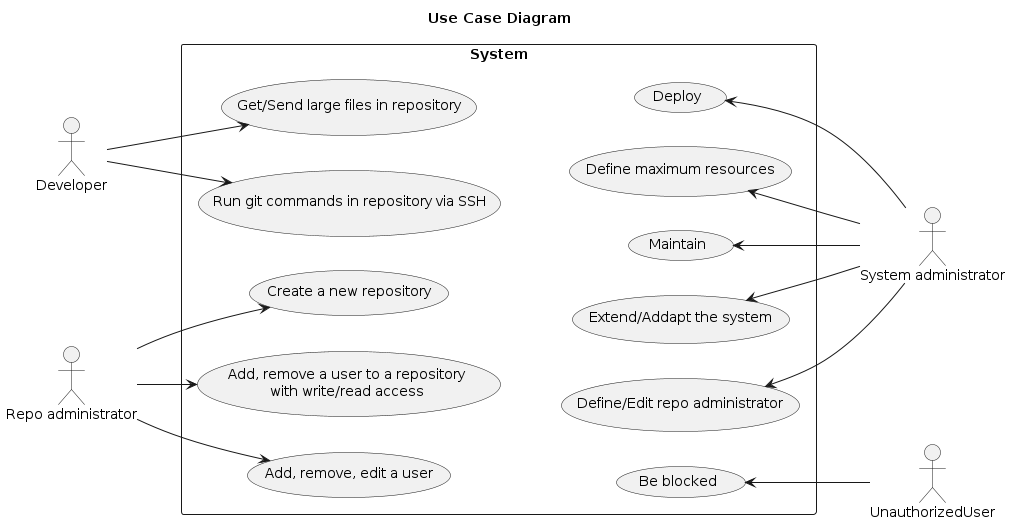
\includegraphics[width=\textwidth]{design/diagrams/use_cases.png}
    \caption{Use cases}
    \label{fig:use_cases}
\end{figure}


\newpage
\section{Scope of the system}

As an example, the system might have the following components. Some components might be reused from existing open-source projects, while others might be developed from scratch.

\begin{itemize}
    \item A git server, behind a ssh server
    \item A git-lfs server, behind a reverse proxy
    \item A storage server
    \item An authentication wrapper
    \item An implementation of the git-lfs-authenticate command
    \item A modifiable configuration of repos and user
\end{itemize}

\paragraph{}
We can draft in figure \ref{fig:architecture} a possible architecture of the system.

\begin{figure}[h]
    \centering
    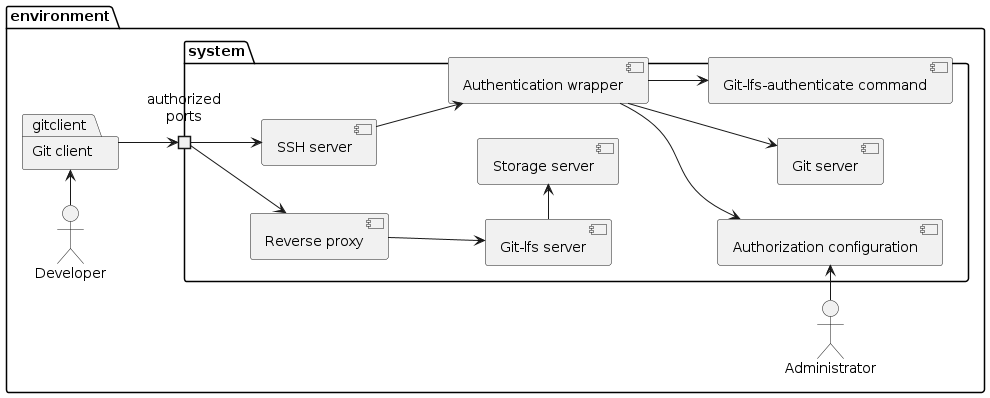
\includegraphics[width=\textwidth]{design/diagrams/context.png}
    \caption{A possible simple architecture of the system, drawing boundaries between the system and the external components}
    \label{fig:architecture}
\end{figure}

\paragraph{}
The fist assumption that we will make it that the git client is not part of the system, nor is the administrator system. However, interfaces to these systems shall be provided.

\paragraph{}
Other organization might only use some components, and make other external components of the system. For example, the storage server will be considered part of the system for this project, but it should be easy to replace it with another storage server, so good interfaces will be provided.

\paragraph{}
To achieve similar features, other projects bundle everything into a single monolith, such as gitlab or gitea, making it impossible to use completely different UI or system based on these. It is possible to use gitlab as a backend for an application based on a different UI, but it is complex to configure and maintain for this use case.  

\newpage
\section{Requirements}

A first analysis leads to the list of requirements of table \ref{tab:requirements}

\begin{table}[h]
    \begin{tabular}{|p{0.1\textwidth}|p{0.4\textwidth}|p{0.15\textwidth}|p{0.25\textwidth}|}
        \hline
        id  & description                                                                                                          & resource                                                                                                 & criterion                                                   \\ \hline
        R1  & The system shall serve all regular git commands (clone, push, pull, etc.).                                           &                                                                                                          & Automated integration testing using common git scenario     \\ \hline
        R2  & The system shall allow for SSH git authentication.                                                                   &                                                                                                          & RSA, ed25519 connexions tests                               \\ \hline
        R3  & The system shall allow for per-repository access control, including read and write access.                           &                                                                                                          & Yes/No                                                      \\ \hline
        R4  & The system shall implement the git-lfs batch/objects API.                                                            & \multirow{2}{*}{\href{https://github.com/git-lfs/git-lfs/blob/main/docs/api/}{specification}} & Automated testing, over 95\% of coverage                    \\ \cline{1-2} \cline{4-4}
        R5  & The system shall implement the git-lfs locks API.                                                                    &                                                                                                          & Automated testing, over 95\% of coverage                    \\ \hline
        R6  & The system shall store LFS files in a separate storage location.                                                     &                                                                                                          & Manual verification of the location of files                \\ \hline
        R7  & Components of the system shall be reusable in other systems.                                                         &                                                                                                          & Several implementations of the file storage shall be tested \\ \hline
        R8  & Only the lock API, the batch API, and the git commands shall be exposed to the outside.                              &                                                                                                          & A deny by default policy must be applied and documented     \\ \hline
        R9  & The system shall be configurable by a single administrator actor (other authorized system or actual person).         &                                                                                                          & A deny by default policy must be applied and documented     \\ \hline
        R10 & The authorization systems shall not share state between the git server and the git-lfs server or the storage server. &                                                                                                          & Yes/No                                                      \\ \hline
        R11 & A first implementation of the system shall be implemented by the end of September 2023                               &                                                                                                          &                                                             \\ \hline
    \end{tabular}
    \caption{Requirements}
    \label{tab:requirements}
\end{table}


\newpage
\section{Functions}

\subsection{Functions identification}

In a first approach, we can identify seven main functions:

\begin{enumerate}
    \item \textbf{Expose api}: the system will expose a public api and prevent access to any private api.
    \item \textbf{Protect git}: the system will authenticate and authorize users to perform git or git-lfs commands.
    \item \textbf{Execute git commands}: the system will execute git commands on behalf of the user, and actually store the repositories in a centralized way.
    \item \textbf{Handle locks}: the system will provide the locking mechanism defined by git-lfs.
    \item \textbf{Protect LFS api}: the system will manage git-lfs requests, mainly verifying that user can upload/download objects
    \item \textbf{Store large objects}: the system will store and retrieve the objects
    \item \textbf{Manage repositories and users}: the system will provide interfaces and mechanisms to manage repositories and users
\end{enumerate}

If we break down these functions one level down, we can identify the sub-functions described by figure \ref{fig:functions}.

\begin{figure}[h]
    \centering
    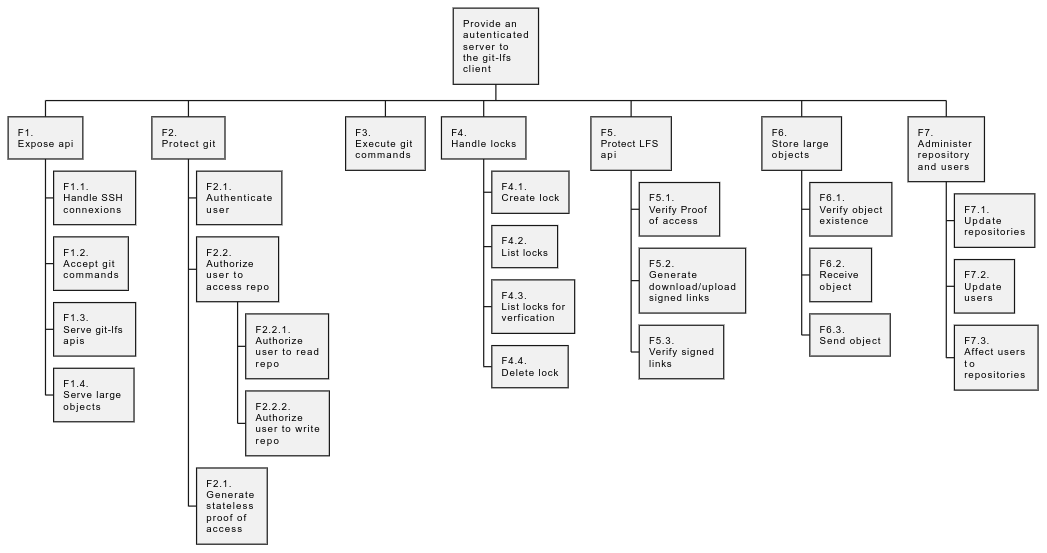
\includegraphics[width=\textwidth]{iteration_00/diagrams/functions.png}
    \caption{Functions}
    \label{fig:functions}
\end{figure}

\subsection{Functions satisfying requirements}

These functions satisfy the requirements of table \ref{tab:requirements}, as shown in the following table:

\begin{longtable}{|p{0.05\textwidth}|p{0.75\textwidth}|p{0.15\textwidth}|}
    \hline
    id  & description                                                                                                          & Satisfied by function \\ \hline
    \endfirsthead
    %
    \endhead
    %
    R1  & The system shall serve all regular git commands (clone, push, pull, etc.).                                           & F3                    \\ \hline
    R2  & The system shall allow for SSH git authentication.                                                                   & F1.1                  \\ \hline
    R3  & The system shall allow for per-repository access control, including read and write access.                           & F7                    \\ \hline
    R4  & The system shall implement the git-lfs batch/objects API.                                                            & F5, F6                \\ \hline
    R5  & The system shall implement the git-lfs locks API.                                                                    & F4                    \\ \hline
    R6  & The system shall store LFS files in a separate storage location.                                                     & F6                    \\ \hline
    R7  & Components of the system shall be reusable in other systems.                                                         & -                     \\ \hline
    R8  & Only the lock API, the batch API, and the git commands shall be exposed to the outside.                              & F1.2, F1.3, F1.4      \\ \hline
    R9  & The system shall be configurable by a single administrator actor (other authorized system or actual person).         & F7                    \\ \hline
    R10 & The authorization systems shall not share state between the git server and the git-lfs server or the storage server. & F2.3, F5              \\ \hline
    R11 & A single implementation of the system shall be implemented by the end of September 2023                              &                       \\ \hline
\end{longtable}

\subsection{Detailed interactions}

As a (too complex) overview, the functions interact with each other as shown in figure \ref{fig:functions_detail}. To break down the complexity, let's consider a few projections of this model.

\begin{figure}[h]
    \centering
    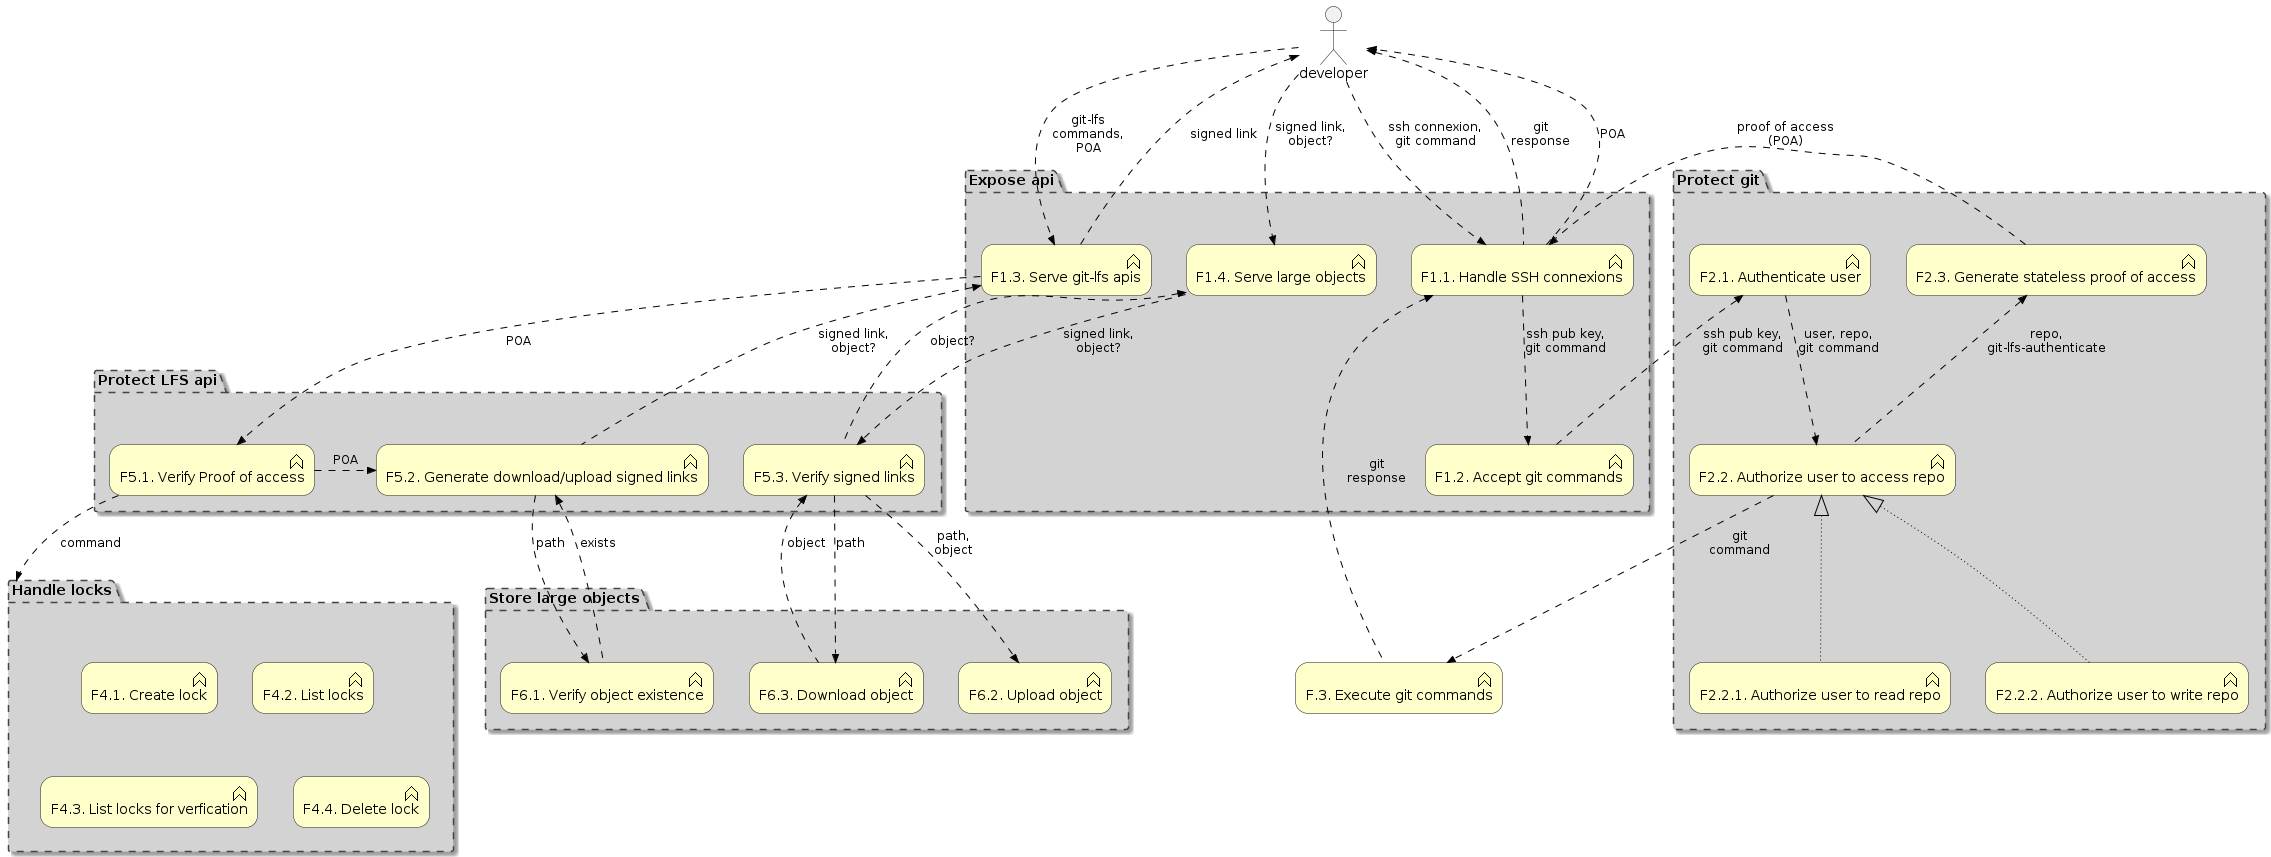
\includegraphics[width=\textwidth]{iteration_00/diagrams/detailed_flow.png}
    \caption{Details of functions interactions}
    \label{fig:functions_detail}
\end{figure}

\subsection{Interactions of first level functions}

At first level, the developer run git commands and get responses. Down, either we go to the git protection functions, and the git functions, or we go to the git-lfs related functions. This separation satisfies R10, as only the stateless proof of access (POA) is shared. User request one to the "git-related" functions, and use it into the "git-lfs" functions. The data flows are shown in figure \ref{fig:functions_overview}

\begin{figure}[h]
    \centering
    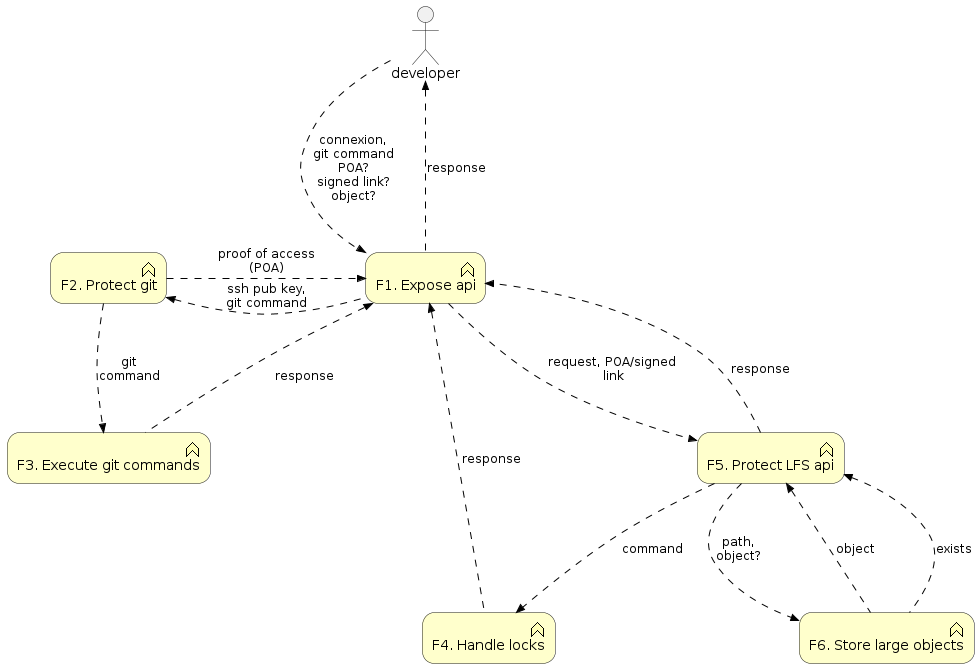
\includegraphics[width=\textwidth]{iteration_00/diagrams/overwiew_flow.png}
    \caption{Overview}
    \label{fig:functions_overview}
\end{figure}

\newpage
\subsection{Regular git flow interactions}

When developer run regular git commands, (no lfs), his SSH connexion must be handled, and then we are ready to accept git commands. But before running them, we shall ensure the uses is allowed to perform them, using the function F2. Then, the git command can be executed and the result be returned to the user via the SSH channel. The whole interaction is shown in figure \ref{fig:simple_git_flow}

\begin{figure}[ht]
    \centering
    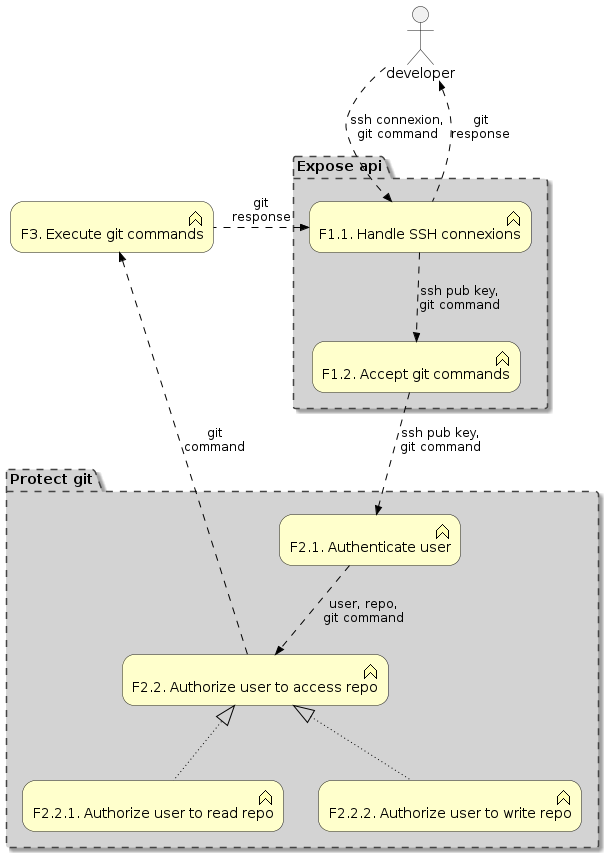
\includegraphics[width=0.6\textwidth]{iteration_00/diagrams/simple_git_flow.png}
    \caption{Simple git flow}
    \label{fig:simple_git_flow}
\end{figure}

\newpage
\subsection{Stateless proof of access flow}

When developer run lfs git commands, he first need to get authenticated. As the lfs functions are unable to access the authorization state of the user, he first need to acquire a proof that he can perform an LFS action. So user first connect through SSH to the authentication server, get a proof of access, and then can use it. The POA acquisition flow is shown in figure \ref{fig:POA_flow}

\begin{figure}[ht]
    \centering
    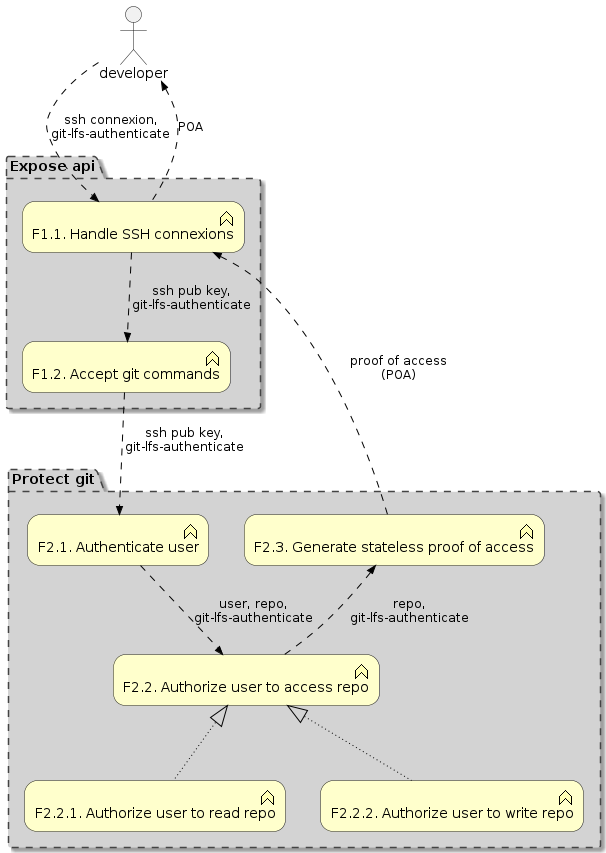
\includegraphics[width=0.6\textwidth]{iteration_00/diagrams/POA_flow.png}
    \caption{POA acquisition flow}
    \label{fig:POA_flow}
\end{figure}

\newpage
\subsection{LFS API flow}

After the user got a POA, he can use it to connect to the LFS api functions, that first verify the POA, and the serve files, locks... The files are also served indirectly, with a stateless signed link, so between requests, no state is saved in the LFS server, even if user can't download all files at once. As defined in the LFS api, the user first request a list of files, get a list of signed links, and the get them one by one. The functions involved in this use of the LFS api are shown in figure \ref{fig:signed_link_flow}

\begin{figure}[ht]
    \centering
    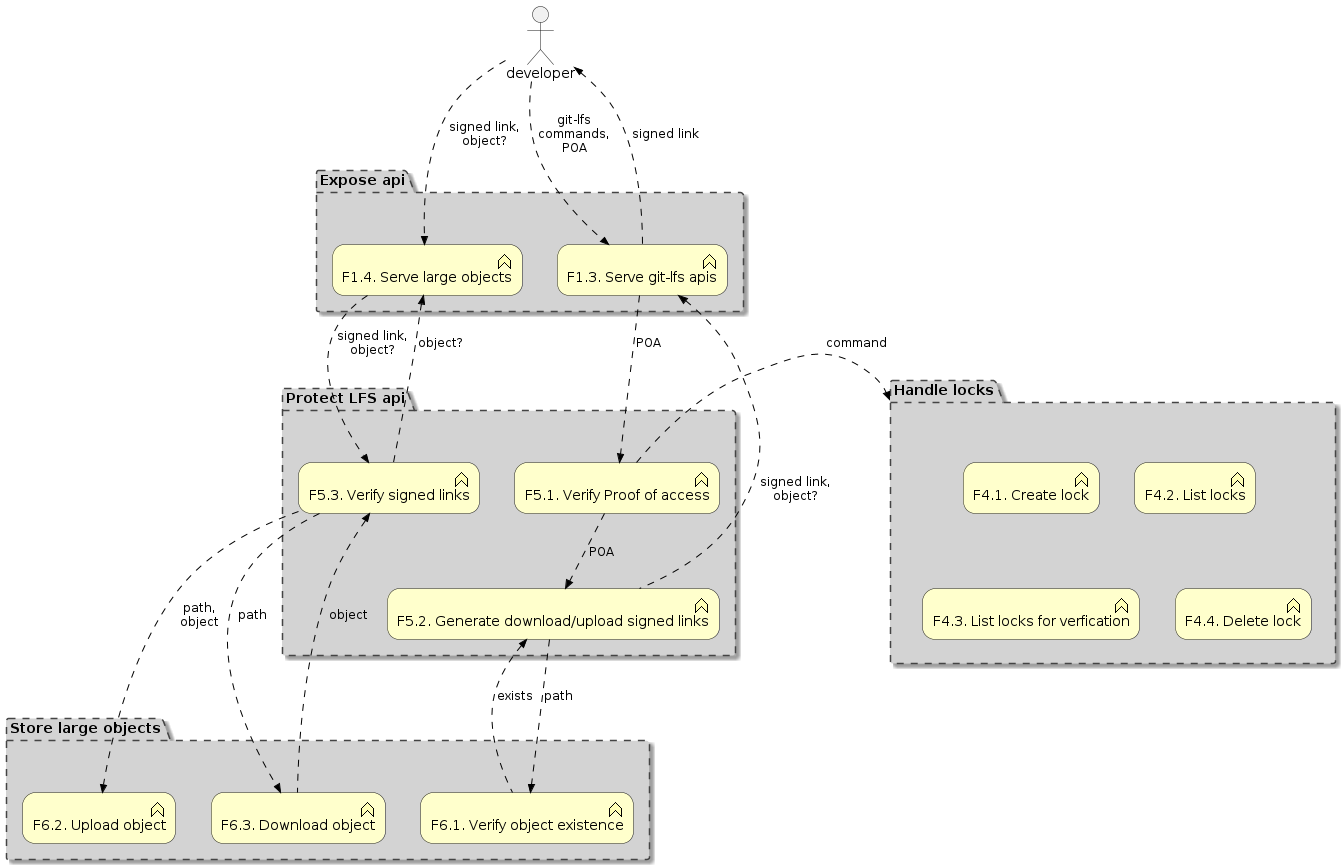
\includegraphics[width=\textwidth]{iteration_00/diagrams/signed_link_flow.png}
    \caption{LFS API flow}
    \label{fig:signed_link_flow}
\end{figure}

\newpage
\section{Components}

As of now, we can guess some of the components that might be used to implement functions.

\begin{figure}[h]
    \centering
    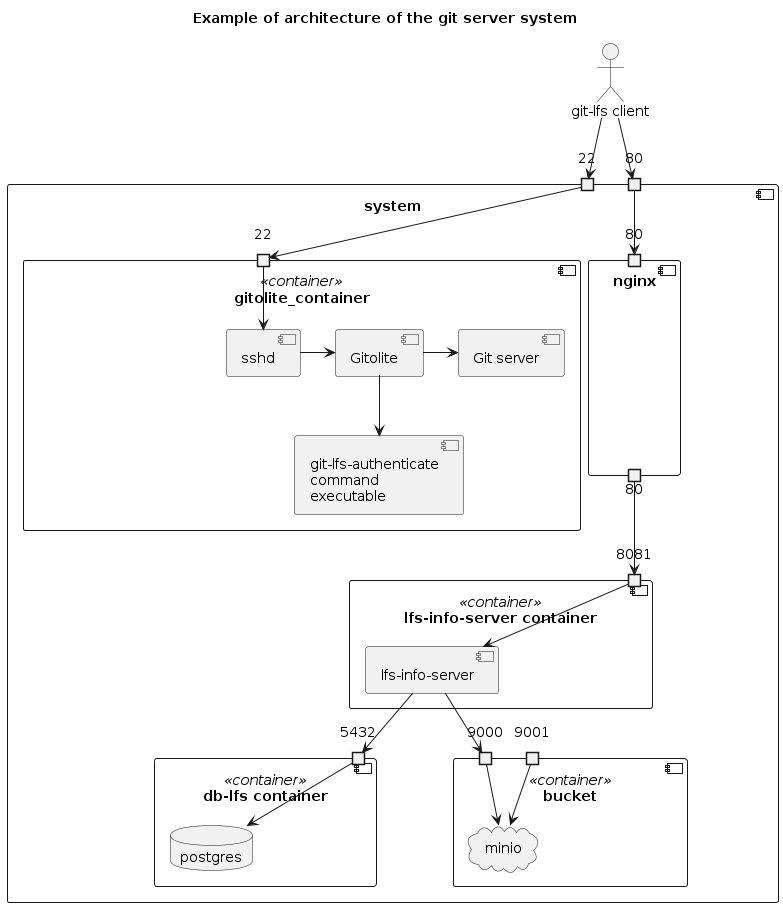
\includegraphics[width=0.8\textwidth]{iteration_01/diagrams/components.png}
    \caption{components}
    \label{fig:components}
\end{figure}

\begin{itemize}
    \item \textbf{F1.1} will be implemented by a sshd server
    \item \textbf{F1.3 and F1.4} Will be implemented by an nginx server, that will act as a reverse proxy for the lfs server.
    \item \textbf{F2.1, F2.2 and F7} will be implemented by  gitolite. It is a git wrapper that allows us to manage users and permissions. A dedicated repository serves as a way to manage to users and repositories.
    \item \textbf{F2.3} will be implemented by a custom git-lfs-authenticate command that will use gitolite to authenticate users by generating the stateless proof of access.
    \item The stateless proof of access shared from \textbf{F2.3 to F5} will be implemented by json web tokens.
    \item \textbf{F3} will be implemented by the git server behind gitolite.
    \item \textbf{F4 and F5} will be implemented by  a custom lfs server that will use MinIO as a storage and postgresql as a database.
    \item \textbf{F6} will be implemented by a MinIO instance, it is a s3 compatible storage.
    \item The components will be containerized using docker and docker-compose
\end{itemize}



\newpage
\part{Life cycle iteration}
\section{Lifecycle derived requirements}

In this part, we will go further by studying the lifecycle of the system. Each step in the live of the product might lead to new questions, new functions, specifications or use cases.

\subsection{Conception}

As a software system, we will most certainly base part of the system on other open-source project. This lead to 2 new requirements: 

\begin{itemize}
    \item \textbf{R12} The system shall use compatible licences, and be loosely coupled enough so the licences of components do not contaminate each other. 
    \item \textbf{R13} The system shall not use deprecated components.
\end{itemize}

\subsection{Deployement}

To minimize costs of the release and deployment cycles, the system shall meet the following requirement:

\begin{itemize}
    \item \textbf{R14} The system shall be deployable in conteneurised linux environments in a reproducible and documented way.  
\end{itemize}

\subsection{Testing}

The \textbf{R14} will also help with testing the system. The system shall be easy to deploy in several instances, as guaranteed by \textbf{R14}

\subsection{Usage}

During usage, performances are key. Each described collaboration takes a few messages in both directions, so time is definitively a concern. To address it, the system shall observe a few more requirements. 

\begin{itemize}
    \item \textbf{R15} Abstraction done of the network layer between the client and the system, the system shall handle an initial push of a 100MB of LFS as 100 large files in less than one minute.  
\end{itemize}

In the opposite direction, the system shall apply limits on the resource used. This will however be dependant on the scale of the deployment, and should then be fine-tuneable

\begin{itemize}
    \item \textbf{R16} The administrator of the system shall be able to define resource limits for the bandwidth, the storage, and the number of requests, separated between the target points (lfs, git), and discriminated by user and repository.
\end{itemize}

This introduce a new actor, the administrator of the system, that is not necessarily the administrator of the repositories and users. 

\subsection{Maintenance}

Many situations can make maintenance a nightmare, but from my experience, a few techniques can radically make things easier: guarantee memory safety, functional correctness, readable code, documentation. 

Therefore, following requirements should be added to the list: 

\begin{itemize}
    \item \textbf{R17} The system shall ensure memory safety and functional correctness either by being heavily maintained by the community, by formal technics, or by automated testing. 
    \item \textbf{R18} Every custom code shall adhere to a common and well-recognized good practices handbook, to be chosen. 
    \item \textbf{R19} The system shall be documented focussing on: the system in its whole, the system components, maintenance processes. 
\end{itemize}

\newpage
\section{Use cases}

In normal use, three types of actors can interact with the system:

\begin{itemize}
    \item \textbf{Developers} are the people that use the system to store and retrieve files. They are authenticated and authorized by the system.
    \item \textbf{Repo administrator} is the people or external system who defines the repositories and the authorizations
    \item \textbf{System administrator} is someone managing the system and its resources. He is owner of the system and defines the system configuration. He maintains and deploy the system.
\end{itemize}

\paragraph{}
Additionally, any non authenticated user is considered harmful and all interactions must be rejected.

\paragraph{}
The figure \ref{fig:use_cases} shows the use cases of these actors of the system. 

\begin{figure}[h]
    \centering
    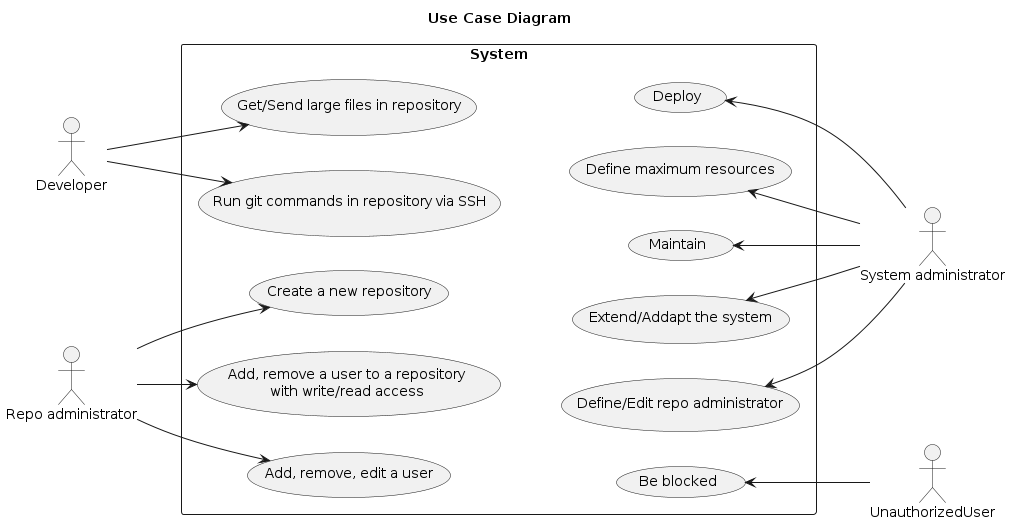
\includegraphics[width=\textwidth]{design/diagrams/use_cases.png}
    \caption{Use cases}
    \label{fig:use_cases}
\end{figure}


\newpage
\section{Sequences}

In this section we will precise the sequences of some use cases.

\subsection{Regular use of git commands}

\paragraph{}
When running regular git commands, the requests of the user pass through a SSH server. His SSH public key serves as an identifier. The SSH server will then forward the request to the authentication and authorization layer, that will forward the command to the git server if the user is authorized to do so. The figure \ref{fig:sequence_git} shows the sequence diagram of this use case.

\begin{figure}[h]
    \centering
    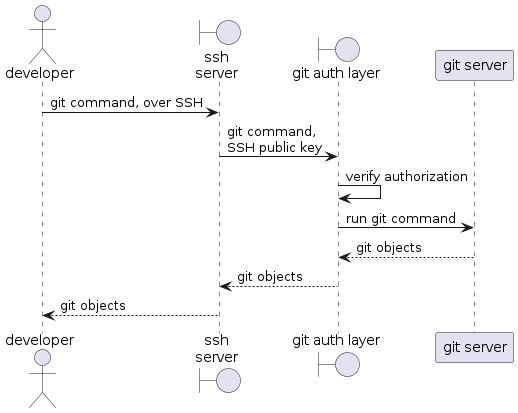
\includegraphics[width=0.7\textwidth]{iteration_01/diagrams/sequence_git.png}
    \caption{Sequence diagram of running a regular git command against the system}
    \label{fig:sequence_git}
\end{figure}

\subsection{LFS commands}

\paragraph{}
In the case of an LFS command, the user first need to get a POA. Then he can request some signed links, and only then upload or download objects. 

\paragraph{}
There is two types of implementation for the links. Either the storage is able to verify these links itself (such as MinIO, or AWS S3), so we can just generate these links and redirect the user to the storage itself; or it does not (such as a regular file system or a NAS), so we need to generate a proxy that will verify the links and then serve the files to the user. Another use of this second implementation would be to reduce the size of the exposed apis: all lfs-related requests would pass through the server, and we don't expose the storage directly to the user. The figure \ref{fig:sequence_lfs} shows the sequence diagram of this use case.


\begin{figure}[ht]
    \centering
    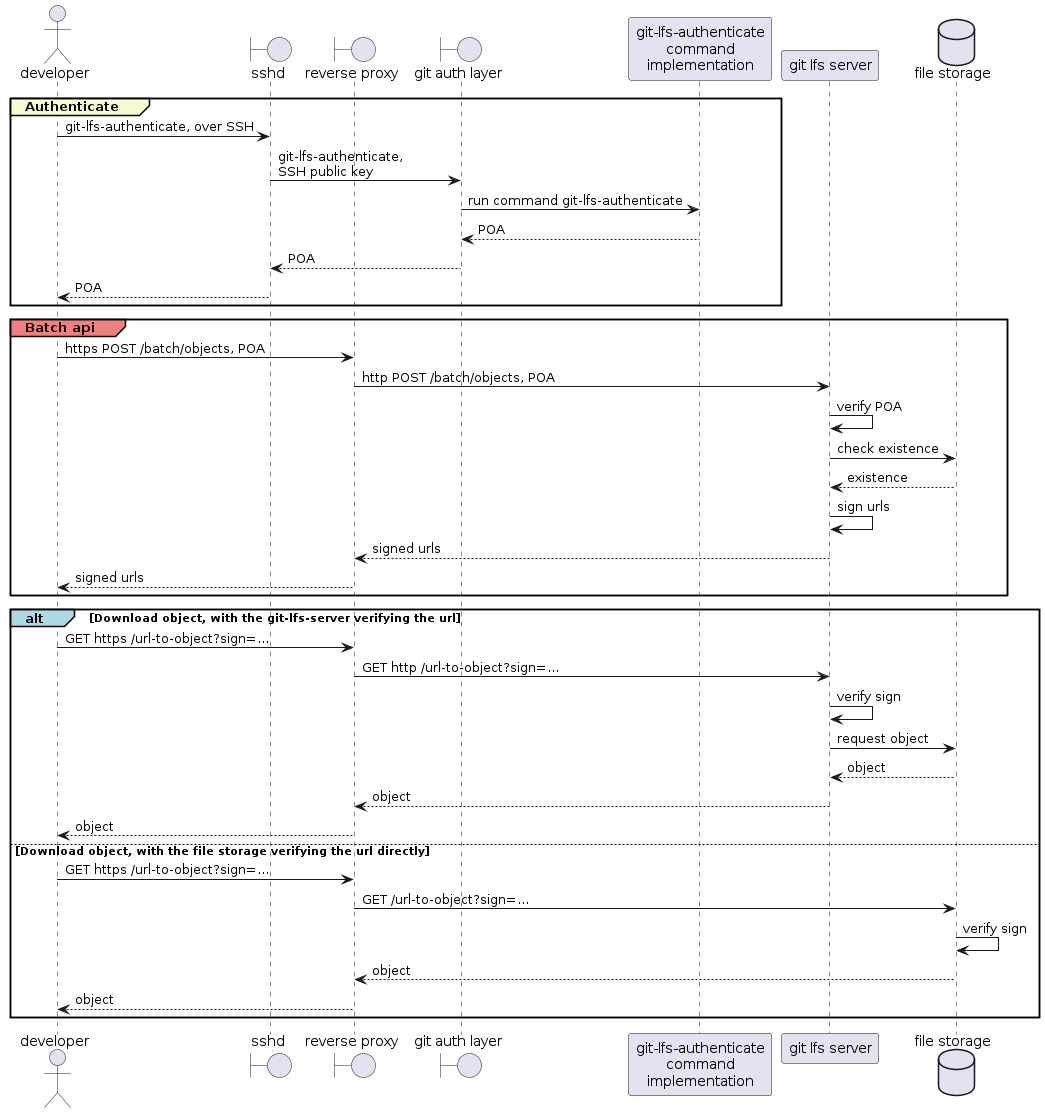
\includegraphics[width=1\textwidth]{iteration_01/diagrams/sequence_lfs.png}
    \caption{Sequence diagram of running lfs git command against the system}
    \label{fig:sequence_lfs}
\end{figure}

\newpage
\section{Requirements}

A first analysis leads to the list of requirements of table \ref{tab:requirements}

\begin{table}[h]
    \begin{tabular}{|p{0.1\textwidth}|p{0.4\textwidth}|p{0.15\textwidth}|p{0.25\textwidth}|}
        \hline
        id  & description                                                                                                          & resource                                                                                                 & criterion                                                   \\ \hline
        R1  & The system shall serve all regular git commands (clone, push, pull, etc.).                                           &                                                                                                          & Automated integration testing using common git scenario     \\ \hline
        R2  & The system shall allow for SSH git authentication.                                                                   &                                                                                                          & RSA, ed25519 connexions tests                               \\ \hline
        R3  & The system shall allow for per-repository access control, including read and write access.                           &                                                                                                          & Yes/No                                                      \\ \hline
        R4  & The system shall implement the git-lfs batch/objects API.                                                            & \multirow{2}{*}{\href{https://github.com/git-lfs/git-lfs/blob/main/docs/api/}{specification}} & Automated testing, over 95\% of coverage                    \\ \cline{1-2} \cline{4-4}
        R5  & The system shall implement the git-lfs locks API.                                                                    &                                                                                                          & Automated testing, over 95\% of coverage                    \\ \hline
        R6  & The system shall store LFS files in a separate storage location.                                                     &                                                                                                          & Manual verification of the location of files                \\ \hline
        R7  & Components of the system shall be reusable in other systems.                                                         &                                                                                                          & Several implementations of the file storage shall be tested \\ \hline
        R8  & Only the lock API, the batch API, and the git commands shall be exposed to the outside.                              &                                                                                                          & A deny by default policy must be applied and documented     \\ \hline
        R9  & The system shall be configurable by a single administrator actor (other authorized system or actual person).         &                                                                                                          & A deny by default policy must be applied and documented     \\ \hline
        R10 & The authorization systems shall not share state between the git server and the git-lfs server or the storage server. &                                                                                                          & Yes/No                                                      \\ \hline
        R11 & A first implementation of the system shall be implemented by the end of September 2023                               &                                                                                                          &                                                             \\ \hline
    \end{tabular}
    \caption{Requirements}
    \label{tab:requirements}
\end{table}


\section{Component Choice}

\subsection{Largely used components}

\paragraph{}
A few components are so largely used that they are almost a standard in the industry. They are used in almost every project and are very well documented. 

\paragraph{}
To handle the SSH connexions (requirement R1.2), the \textit{sshd} deamon is used. It is the standard SSH server for Linux using the OpenSSH implementation of SSH. It is very well documented and is used in almost every Linux distribution. It supports the SSH protocol version 1 and 2. 

\paragraph{}
To conteneurise the application (requirement R4.1), Docker is used. It is also now a standard in the industry. Docker-compose can be used to describe the containers and their interactions. 

\paragraph{}
To expose ports in a secure way (requirement R4.2), we can leverage containers to only expose the ports we want to expose, then use a reverse proxy to expose the containers. This way, we can have a single entry point to the application and we can easily add rate limitations and protections. A standard reverse proxy is Nginx, that can be configured with a single file, to satisfy the requirement R4.

\paragraph{}
To handle stateless proofs of access (requirement R4.3), we can use JWT tokens. Their security has been proven and they allow for json complex payload.

\paragraph{}
Storages (requirement R2.2) can be handled by a MinIO instance, a local file storage, databases. As discussed previously, the storage is often one of the component the organizations want to keep control of, so several implementations will be available.

\paragraph{}
To handle git commands, nothing best than the git command line tool. It is already a server and is the reference, production ready implementation of git. 

\paragraph{}
At this point, if we go back to the components view, in green are colored the components that are now well defined. 

% side by side images in figure
\begin{figure}[H]
    \centering
    \begin{minipage}{.5\textwidth}
        \centering
        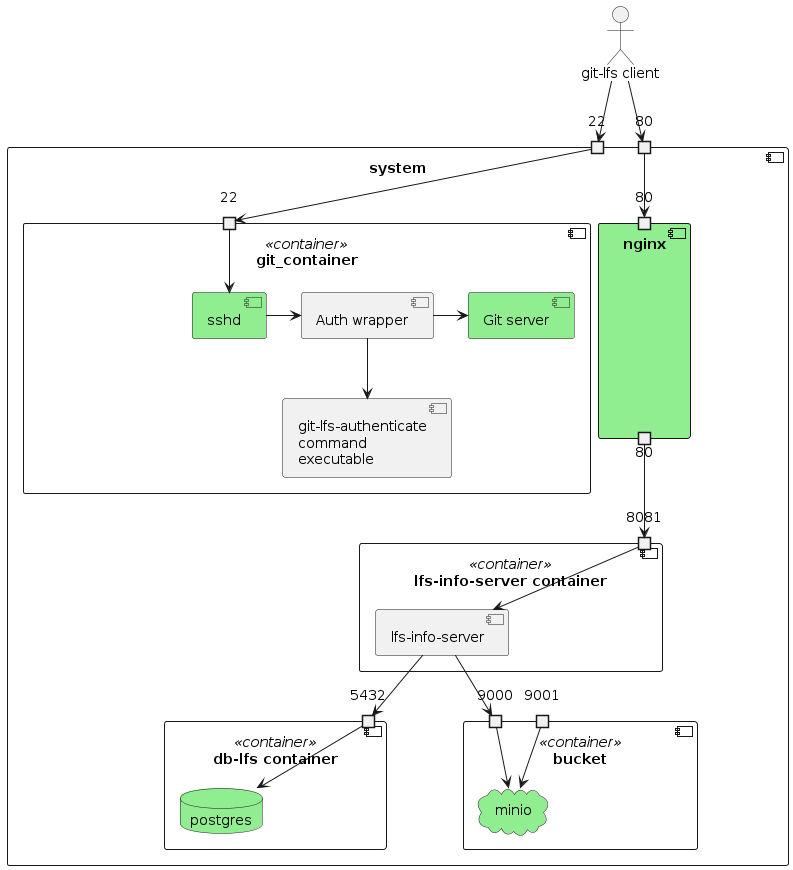
\includegraphics[width=0.95\linewidth]{iteration_01/diagrams/components_chosen_1.png}
        \caption{Components}
        \label{fig:components_chosen_1}
    \end{minipage}%
    \begin{minipage}{.5\textwidth}
        \centering
        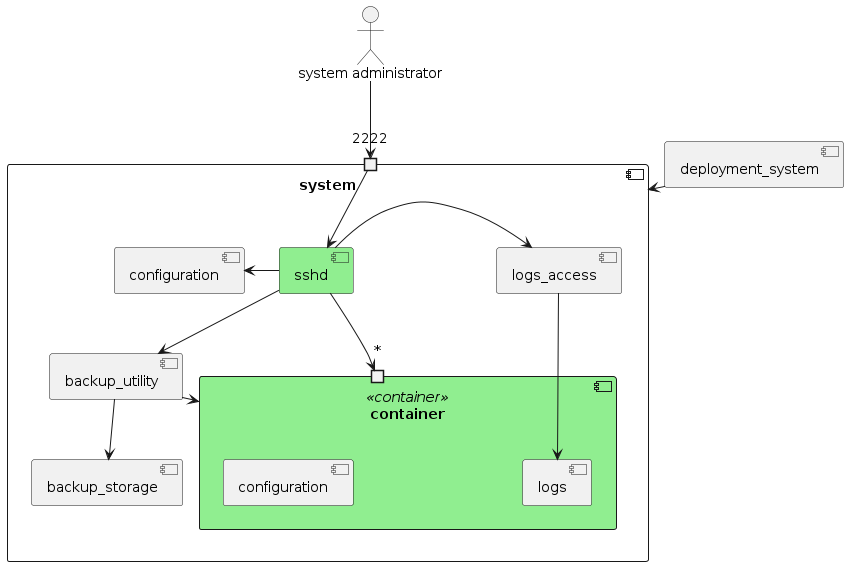
\includegraphics[width=0.95\linewidth]{iteration_01/diagrams/components_chosen_2.png}
        \caption{Components}
        \label{fig:components_chosen_2}
    \end{minipage}
\end{figure}

\subsection{Git wrapper}

To bring the authentication and authorization layer to git, two solutions are possible. 

\paragraph{}
The first one is to use unix permissions and allow users to run git command (and only git commands) directly through SSH. If they push to an authorized location, the push will be accepted. If they push to an unauthorized location, the push will be rejected. This solution seems simple, but managing hundreds or thousands of users on a single server using only unix permissions is hard to do right. The developpment of a custom solution would be required. Auditing history of permissions changes would not be possible without another layer.  

\paragraph{}
The single solution, addopted by almost every large actor (Github, Gitlab, Bitbucket, etc.) is to create a single git user. Then all users add their public keys, and when they login, their key is verified, and they are identified by them. A very clever implementation of these mechanisms is provided by Gitolite. It is a git server that allows to manage users and their permissions using a git repository. It is very well documented and is used for instance the KDE project, the Fedora project, kernel.org, gentoo linux, etc.

\paragraph{}
Gitolite would satisfy a lot of requirements:

\begin{itemize}
    \item R1.1: Gitolite expose a gitolite-shell command line that proxy git commands to the git server, so all regular git commands are available.
    \item R1.2: Gitolite is put just behind the SSH server
    \item R2.1 and 2.4: Gitolite defines a repository "gitolite-admin" that contain all the public keys of users, and a list of repositories, with each user having read or write access to each of them. Changing permissions is a simple as modifying this file and pushing modification. 
    \item R2.5: gitolite is under the GPL v2 license, allowing for commercial use, modification and distribution. However it contaminates the code that uses it with the GPL license. Using it will therefore require good separations between this component and other components that might need to be modified by enterprises in a proprietary way.
    \item R2.6: gitolite is still very active (last commit was 2 months ago, there are 38 contributors, 8.2k stars on github, and 1k forks)
    \item R3.2: the system is heavily used and tested, and might be considered very stable.
\end{itemize}

\paragraph{}
Gitolite also allow for custom commands to be injected in the system. It would then be possible to implement the \textit{git-lfs-authenticate} command inside gitolite, in rust, getting gitolite to verify the user, signing the JWT, and returning it to the client for later use. Such a simple command can be done in a few hours. 

\paragraph{}
Remains one of the big part: the git lfs server, that is not handled by gitolite.

\subsection{Git LFS server implementations}
The git lfs team list a few implementations of their protocol on \url{https://github.com/git-lfs/git-lfs/wiki/Implementations}

However, most of them do not match our requirements:

\begin{itemize}
    \item \textit{jasonwhite/rudolfs} lacks authentication, not even supporting jwt
    \item \textit{git-lfs/lfs-test-server}, \textit{cloudmazing/lfs-server-go} are not production ready
    \item \textit{artemkin/git-lfs-server}, \textit{cbartz/git-lfs-swift}, \textit{meltingice/git-lfs-s3}, \textit{mgax/lfs}, \textit{kzwang/node-git-lfs} are deprecated or unmaintained
    \item \textit{bozaro/git-as-svn} and \textit{saracen/lfscache} are out of scope, they primarily focus on caching, or making git work like svn. 
    \item \textit{charmbracelet/git-lfs-transfer} and \textit{autovia/git-lfs-transfer} are exploratory works of lfs over ssh, but are not compatible with regular git lfs clients
    \item \textit{metalogical/BigFiles}, \textit{gitlit}, \textit{AKSW/git\_lfs\_server\_sshauth}, \textit{khoa-io/git-lfs}, \textit{alanedwardes/Estranged.Lfs} are only partial implementations of the API
    \item \textit{OneDev}, \textit{GitBucket}, \textit{Gitea}, \textit{GitLab}, \textit{Gitblit}, \textit{SCM-Manager} are full git platforms, so too high level to be used as foundation for custom enterprise solutions
\end{itemize}

\paragraph{}
It remains two solutions to investigate

\begin{itemize}
    \item \textit{bozaro/git-lfs-java} is a Java implementation that supports locks, objects batch apis. It defines no implementation though, but it might be possible to implement them in Java. However, last human commit was one year ago, and the project is not very used. The project is licenced under the LGPL v3 license, allowing for commercial use, modification and distribution. However it contaminates the code that uses it with the LGPL license.
    \item \textit{datopian/giftless} support basic transfer, S3 backend storage, and jwt authentication. It is written in python. It is a little more used (25 forks and 85 stars)
\end{itemize}

\paragraph{}
Both implementations will need to be extended, and the git-lfs-java will be hard to extends legally, and safely, as rust will not be an option. The giftless implementation is more promising, but present few garanties of performance and stability. This server will be a part of the system that would benefit the most from a custom implementation that is stable, performant, and that can be modified by enterprises in a proprietary way.

\newpage
\section{Git LFS Server}

\paragraph{}
As discussed, we need to implement a git lfs server that match our requirements. One of the most complex one is reusability and modularity with several storage backends.

\subsection{Storage backends and services injections}

\paragraph{}
The figure \ref{fig:lfs_server_all_enabled} shows the architecture of the git lfs server services. Three apis are exposed:

\begin{itemize}
    \item The objects batch api, to request links that will be used to upload and download objects.
    \item The file api, to actually upload and download objects
    \item The locks api.
\end{itemize}

\begin{figure}[H]
    \centering
    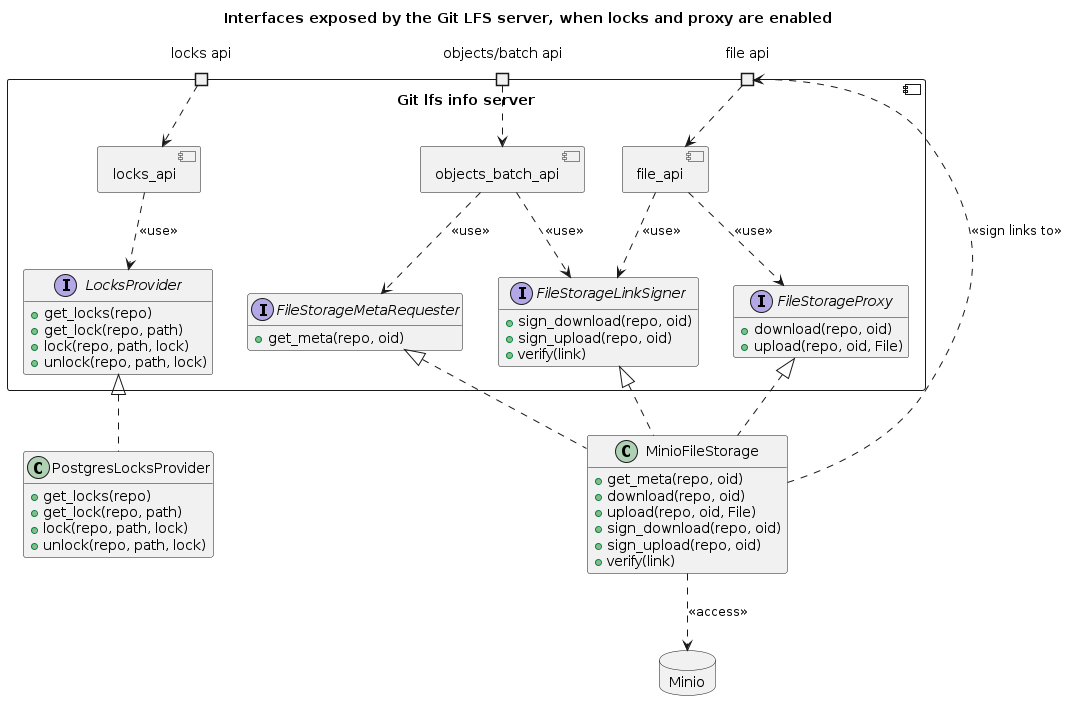
\includegraphics[width=0.95\linewidth]{iteration_01/diagrams/lfs_server_all_enabled.png}
    \caption{Git LFS Server}
    \label{fig:lfs_server_all_enabled}
\end{figure}

\paragraph{}
In this mode, all apis are enabled, and two classes implement the storage backend interfaces, using postgresql for locks and minio for files.

\paragraph{}
On the other hand, one might not need the locks api, or might implement a link signer that redirect directly to the storage server. In that case, not all interfaces will be injected, and considering only the ones that are, the system will look like the figure \ref{fig:lfs_server_minimal}.

\begin{figure}[H]
    \centering
    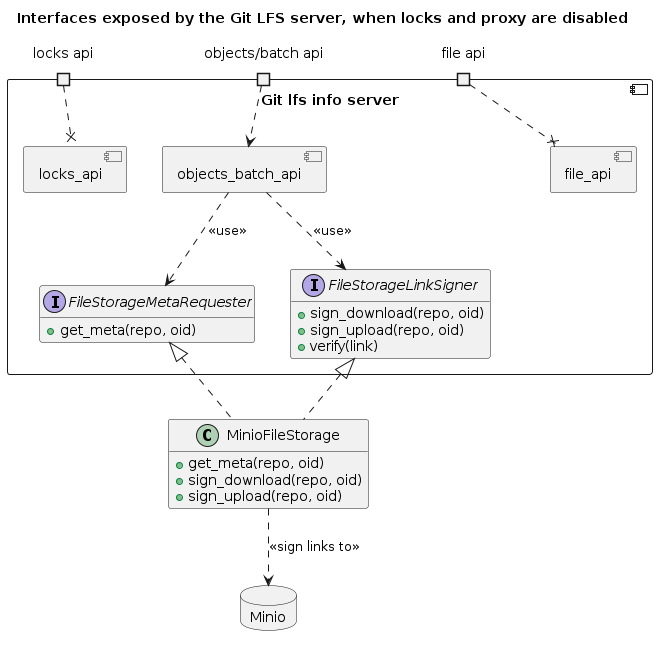
\includegraphics[width=0.95\linewidth]{iteration_01/diagrams/lfs_server_minimal.png}
    \caption{Git LFS Server}
    \label{fig:lfs_server_minimal}
\end{figure}

\subsection{Locks api requirements}

The requirement \textbf{R1.4} can be further derived from the official specification into:

\begin{itemize}
    \item \textbf{R1.4.1}: the server shall expose a `POST /locks` route, accepting a payload with a repo name, a path, and a ref, that create a lock for the path, the ref, and the repo, and mark user as the owner of the lock.
    \item \textbf{R1.4.2}: the server shall respond to a lock creation either by returning the lock, by a "bad response, lock exists" response, including the existing lock
    \item \textbf{R1.4.3}: the server shall expose a `GET /locks` route, accepting a payload with optional paths, id, refspec; it shall match all corresponding locks and return them.
    \item \textbf{R1.4.4}: the server shall expose a `POST /locks/verify` route, accepting a payload with an optional ref name, and locks separated between \textit{ours} (the locks of user) and \textit{theirs} (the locks of teammates)
    \item \textbf{R1.4.5}: the server shall accept cursor, limit in the `GET /locks` and `POST /locks/verify` payload, so it selects at most \textit{limit} locks, starting at \textit{cursor}. It shall return the next cursor if there are more than \textit{limit} locks
    \item \textbf{R1.4.6}: the server shall expose a `POST /locks/:id/unlock`, that delete the lock by id and return it.
    \item \textbf{R1.4.7}: the server shall verify that user deleting a lock is owner of the lock. If he is not, the deletion shall only occur if an attribute `force:true` is passed in the payload.
    \item \textbf{R1.4.8}: the server shall verify that user has the right to write the repository, checking for the json web token
    \item \textbf{R1.4.9}: for all routes, in the event of an error, the server shall return an error response as a JSON containing a message property.
    \item \textbf{R1.4.10}: any route shall respect the schemas defined in the \url{https://github.com/git-lfs/git-lfs/blob/main/docs/api/locking.md}
\end{itemize}

\subsection{Batch api requirements}

\paragraph{}

The requirement \textbf{R1.3} can be further derived from the official specification into:

\begin{itemize}
    \item \textbf{R1.3.1}: the server shall accept a get request on route /objects/batch?repo=... with payload matching the payload from \url{https://github.com/git-lfs/git-lfs/blob/main/docs/api/batch.md#requests}
    \item \textbf{R1.3.2}: the server shall return for route objects\_batch the operation, the hash\_algo, and an array of objects containing presigned links to perform a download/upload operation, according to the \url{https://github.com/git-lfs/git-lfs/blob/main/docs/api/batch.md#successful-responses}
    \item \textbf{R1.3.3}: In case of error generating the link, the error returned should be embedded into the response (the request shall not fail) according to the \url{https://github.com/git-lfs/git-lfs/blob/main/docs/api/batch.md#successful-responses}. The error shall be one of
          \begin{itemize}
              \item \textit{404}: The object does not exist on the server.
              \item \textit{409}: The specified hash algorithm disagrees with the server's acceptable options.
              \item \textit{410}: The object was removed by the owner.
              \item \textit{422}: Validation error.
          \end{itemize}
    \item \textbf{R1.3.4}: In case of failure leading to global failure of the request, the server shall return the appropriate HTTP status code and a json object containing a message property. Only the following errors shall happen:
          \begin{itemize}
              \item \textit{401}: The authentication credentials are needed, but were not sent. Git LFS will attempt to get the authentication for the request and retry immediately.
              \item \textit{403}: The user has read, but not write access. Only applicable when the operation in the request is "upload."
              \item \textit{404}: The Repository does not exist for the user.
              \item \textit{422}: Validation error with one or more of the objects in the request. This means that none of the requested objects to upload are valid.
              \item \textit{406}: The Accept header needs to be application/vnd.git-lfs+json.
              \item \textit{413}: The batch API request contained too many objects or the request was otherwise too large.
              \item \textit{429}: The user has hit a rate limit with the server. Though the API does not specify any rate limits, implementors are encouraged to set some for availability reasons.
              \item \textit{501}: The server has not implemented the current method. Reserved for future use.
              \item \textit{507}: The server has insufficient storage capacity to complete the request.
              \item \textit{509}: The bandwidth limit for the user or repository has been exceeded. The API does not specify any bandwidth limit, but implementors may track usage.
              \item \textit{500}: Any other server error
          \end{itemize}
\end{itemize}


\newpage


\newgeometry{margin=1cm}
\begin{landscape}
    {
        \titleformat{\section}
  {\normalfont\Large\bfseries}{\llap{\parbox{0em}{\thesection\hfill}}}{3em}{}

        \section{Requirements table}
        
    }
    
    \begin{longtable}{|p{1cm}|p{19cm}|p{2cm}|p{3cm}|}
        \hline
        \rowcolor[HTML]{9B9B9B}
        id                                  & description                                                                                                                                                                                                                                                                           & Satisfied by function & Implemented by component                 \\ \hline
        \endfirsthead
        %
        \endhead
        %
        \rowcolor[HTML]{C0C0C0}        R1   & The system shall implement git and git-lfs repositories over SSH.                                                                                                                                                                                                                     &                       &                                          \\ \hline
        \rowcolor[HTML]{DDDDDD}        R1.1 & The system shall serve all regular git commands (clone, push, pull, etc.).                                                                                                                                                                                                            & F1.2, F3              & Git server                               \\ \hline
        \rowcolor[HTML]{DDDDDD}        R1.2 & The system shall allow for SSH git authentication.                                                                                                                                                                                                                                    & F1.1                  & sshd, gitolite                           \\ \hline
        \rowcolor[HTML]{DDDDDD}        R1.3 & The system shall implement the git-lfs batch/objects API.                                                                                                                                                                                                                             & F1.3                  & git lfs server                           \\ \hline
        R1.3.1                              & the server shall accept a get request on route /objects/batch?repo=... with payload matching the payload from \url{https://github.com/git-lfs/git-lfs/blob/main/docs/api/batch.md#requests}                                                                                           &                       &                                          \\\hline
        R1.3.2                              & the server shall return for route objects\_batch the operation, the hash\_algo, and an array of objects containing presigned links to perform a download/upload operation, according to the \url{https://github.com/git-lfs/git-lfs/blob/main/docs/api/batch.md#successful-responses} &                       &                                          \\\hline
        R1.3.3                              & In case of error generating the link, the error returned should be embedded into the response (the request shall not fail) according to the \url{https://github.com/git-lfs/git-lfs/blob/main/docs/api/batch.md#successful-responses}. The error shall be one of                      &                       &                                          \\\hline
        R1.3.4                              & In case of failure leading to global failure of the request, the server shall return the appropriate HTTP status code and a json object containing a message property. Only the following errors shall happen:                                                                        &                       &                                          \\\hline
        \rowcolor[HTML]{DDDDDD}        R1.4 & The system shall implement the git-lfs locks API.                                                                                                                                                                                                                                     & F1.4                  & Git lfs server                           \\ \hline
        R1.4.1                              & the server shall expose a `POST /locks` route, accepting a payload with a repo name, a path, and a ref, that create a lock for the path, the ref, and the repo, and mark user as the owner of the lock.                                                                               &                       &                                          \\\hline
        R1.4.2                              & the server shall respond to a lock creation either by returning the lock, by a "bad response, lock exists" response, including the existing lock                                                                                                                                      &                       &                                          \\\hline
        R1.4.3                              & the server shall expose a `GET /locks` route, accepting a payload with optional paths, id, refspec; it shall match all corresponding locks and return them.                                                                                                                           &                       &                                          \\\hline
        R1.4.4                              & the server shall expose a `POST /locks/verify` route, accepting a payload with an optional ref name, and locks separated between \textit{ours} (the locks of user) and \textit{theirs} (the locks of teammates)                                                                       &                       &                                          \\\hline
        R1.4.5                              & the server shall accept cursor, limit in the `GET /locks` and `POST /locks/verify` payload, so it selects at most \textit{limit} locks, starting at \textit{cursor}. It shall return the next cursor if there are more than \textit{limit} locks                                      &                       &                                          \\\hline
        R1.4.6                              & the server shall expose a `POST /locks/:id/unlock`, that delete the lock by id and return it.                                                                                                                                                                                         &                       &                                          \\\hline
        R1.4.7                              & the server shall verify that user deleting a lock is owner of the lock. If he is not, the deletion shall only occur if an attribute `force:true` is passed in the payload.                                                                                                            &                       &                                          \\\hline
        R1.4.8                              & the server shall verify that user has the right to write the repository, checking for the json web token                                                                                                                                                                              &                       &                                          \\\hline
        R1.4.9                              & for all routes, in the event of an error, the server shall return an error response as a JSON containing a message property.                                                                                                                                                          &                       &                                          \\\hline
        R1.4.10                             & any route shall respect the schemas defined in the \url{https://github.com/git-lfs/git-lfs/blob/main/docs/api/locking.md}                                                                                                                                                             &                       &                                          \\\hline
        \rowcolor[HTML]{C0C0C0}        R2   & The system shall be usable as a low-level foundation for commercial and non-commercial multi-users applications based around git repositories.                                                                                                                                        &                       &                                          \\ \hline
        \rowcolor[HTML]{DDDDDD}        R2.1 & The system shall allow for per-repository access control, including read and write access.                                                                                                                                                                                            & F2                    & Gitolite                                 \\ \hline
        R2.1.1                              & The authentication and authorization subsystem shall be able to verify if a given user has read or write access to a given repository.                                                                                                                                                &                       &                                          \\ \hline
        R2.1.2                              & The authentication and authorization subsystem shall expose a command named \textit{git-lfs-authenticate}, which will return a json web token signing the user, the repository, the operation, and the expiration date.                                                               &                       &                                          \\ \hline
        R2.1.3                              & The lfs server shall accept and verify a json web token signing the user, the repository, the operation, and the expiration date.                                                                                                                                                     & F5.1                  &                                          \\ \hline
        R2.1.4                              & The lfs server shall be able to generate a signed link for a given file, operation, and expiration date that can't be modified by the user.                                                                                                                                           & F5.2                  &                                          \\ \hline
        R2.1.5                              & The file server (either the lsf info server acting as a proxy or the storage server directly) shall be able to verify a signed link for a given file, operation, and expiration date, and serve or accept the requested file, depending on the operation.                             & F5.3                  &                                          \\ \hline
        \rowcolor[HTML]{DDDDDD}        R2.2 & The system shall store data files in a separate storage location.                                                                                                                                                                                                                     &                       & Postgres, Minio                          \\ \hline
        R2.2.1                              & The system shall implement the storage interfaces of \textbf{R2.3.1} for the MinIO API, using a Single Bucket Storage policy (SBS)                                                                                                                                                    & F6                    &                                          \\\hline
        R2.2.2                              & The system shall implement the storage interfaces of \textbf{R2.3.1} for the local file system API                                                                                                                                                                                    & F6                    &                                          \\\hline
        R2.2.3                              & The system shall implement the lock storage interfaces of \textbf{R2.3.3} for the MinIO API, using a Single Bucket Storage policy (SBS)                                                                                                                                               & F4                    &                                          \\\hline
        R2.2.4                              & The system shall implement the lock storage interfaces of \textbf{R2.3.3} for postgresql database                                                                                                                                                                                     & F4                    &                                          \\\hline
        \rowcolor[HTML]{DDDDDD}        R2.3 & Components of the system shall be reusable in other systems.                                                                                                                                                                                                                          &                       &                                          \\ \hline
        R2.3.1                              & The system shall define file storage interfaces, to retrieve metadata about a file, to retrieve a file, and to store a file.                                                                                                                                                          & F6                    &                                          \\\hline
        R2.3.2                              & The system shall model implementations of the storage interfaces of \textbf{R2.3.1} for other storages: Multiple Bucket Storage policy (MBS), and File Transfer Protocol (FTP), and local storage with database stored metadata (LSDB)                                                & F6                    &                                          \\\hline
        R2.3.3                              & The system shall define lock storage interfaces, to create, list, and delete locks.                                                                                                                                                                                                   & F4                    &                                          \\\hline
        R2.3.4                              & The system shall model implementations of the lock storage interfaces of \textbf{R2.3.3} for other storages: Locks in multiple buckets (LMB), Locks in local file storage.                                                                                                            & F4                    &                                          \\\hline
        \rowcolor[HTML]{DDDDDD}        R2.4 & The system repositories and users shall be configurable by a single administrator actor (other authorized system or actual person).                                                                                                                                                   & F7                    & Gitolite                                 \\ \hline
        \rowcolor[HTML]{DDDDDD}        R2.5 & The system shall use compatible licences, and be loosely coupled enough so the licences of components do not contaminate each other.                                                                                                                                                  &                       &                                          \\ \hline
        \rowcolor[HTML]{DDDDDD}        R2.6 & The system shall not use deprecated components.                                                                                                                                                                                                                                       &                       &                                          \\ \hline
        \rowcolor[HTML]{DDDDDD}        R2.7 & Abstraction done of the network layer between the client and the system, the system shall handle an initial push of a 100MB of LFS as 100 large files in less than one minute.                                                                                                        &                       &                                          \\ \hline
        \rowcolor[HTML]{C0C0C0}        R3   & The system shall be developed in 200 hours-man by the end of October 2023, and require at most 100 hours-man per year to be maintained by the community..                                                                                                                             &                       &                                          \\ \hline
        \rowcolor[HTML]{DDDDDD}        R3.1 & A first implementation of the system shall be implemented by the end of September 2023                                                                                                                                                                                                &                       &                                          \\ \hline
        \rowcolor[HTML]{DDDDDD}        R3.2 & The system shall ensure memory safety and functional correctness either by being heavily maintained by the community, by formal technics, or by automated testing.                                                                                                                    &                       &                                          \\ \hline
        R3.2.1                              & Custom parts of the system shall be implemented in the rust programming language.                                                                                                                                                                                                     &                       & git-lfs-authenticate command; lfs server \\\hline
        R3.2.2                              & Non custom parts of the system shall be heavily adopted by the community to be considered safe.                                                                                                                                                                                       &                       & gitolite, git, nginx, ...                \\\hline
        R3.2.3                              & Custom parts of the system shall be tested using automated testing, with a coverage of at least 90\%.                                                                                                                                                                                 &                       & git-lfs-authenticate command; lfs server \\\hline
        \rowcolor[HTML]{DDDDDD}        R3.3 & Every custom code shall adhere to a common and well-recognized good practices handbook, to be chosen.                                                                                                                                                                                 &                       & git-lfs-authenticate command; lfs server \\ \hline
        R3.3.1                              & Custom apis of the system should adhere to the following good practices handbooks \url{https://rust-lang.github.io/api-guidelines/}, \url{https://cheats.rs/#idiomatic-rust} and \url{https://rust-unofficial.github.io/patterns/}                                                    &                       &                                          \\\hline
        R3.3.2                              & Custom code of the system shall use the linter \url{https://github.com/rust-lang/rust-clippy}                                                                                                                                                                                         &                       &                                          \\\hline
        \rowcolor[HTML]{DDDDDD}        R3.4 & The system shall be documented focussing on: the system in its whole, the system components, maintenance processes.                                                                                                                                                                   &                       &                                          \\ \hline
        R3.4.1                              & Every custom and non-custom code of the system shall be documented in term of context and role in the system, and in term of possible replacements.                                                                                                                                   &                       &                                          \\\hline
        R3.4.2                              & The system shall be documented in term of architecture, and in term of maintenance processes.                                                                                                                                                                                         &                       &                                          \\\hline
        R3.4.3                              & The system shall be documented in term of deployment processes.                                                                                                                                                                                                                       &                       &                                          \\\hline
        R3.4.4                              & Custom code of the system shall be documented in term of technical choices and design.                                                                                                                                                                                                &                       &                                          \\\hline
        \rowcolor[HTML]{C0C0C0}        R4   & The system shall be deployable in less than 1h in an enterprise-grade environment.                                                                                                                                                                                                    &                       &                                          \\ \hline
        \rowcolor[HTML]{DDDDDD}        R4.1 & The system shall be deployable in conteneurised linux environments in a reproducible and documented way.                                                                                                                                                                              &                       & Docker, docker-compose                   \\ \hline
        \rowcolor[HTML]{DDDDDD}        R4.2 & Only the lock API, the batch API, and the git commands shall be exposed to the outside.                                                                                                                                                                                               &                       & Nginx                                    \\ \hline
        \rowcolor[HTML]{DDDDDD}        R4.3 & The authorization systems shall not share state between the git server and the git-lfs server or the storage server.                                                                                                                                                                  &                       & git-lfs authenticate command, lfs server \\ \hline
        \rowcolor[HTML]{DDDDDD}        R4.4 & The administrator of the system shall be able to define resource limits for the bandwidth, the storage, and the number of requests, separated between the target points (lfs, git), and discriminated by user and repository.                                                         &                       &                                          \\ \hline
        \rowcolor[HTML]{DDDDDD}        R4.5 & The system shall do regular backups of the data.                                                                                                                                                                                                                                      &                       &                                          \\ \hline
    \end{longtable}
\end{landscape}

\titleformat{\section}
  {\normalfont\Large\bfseries}{\llap{\parbox{\titleindent}{\thesection\hfill}}}{0em}{}

  \newgeometry{left=3cm,right=3cm,top=3cm,bottom=5cm}


\section{Conclusion}
Further modeling will take place as this project move forward, but this document presented the start of the conception process of the system.

Next steps would be:

\begin{itemize}
    \item To get some feedback about the achieved requirements
    \item To push further the behavior views (mainly activity/sequence diagrams) to further specify and document the logic behind the object and locks api.
    \item To implement
\end{itemize}

\end{document}
